\section{define.h File Reference}
\label{define_8h}\index{define.h@{define.h}}
{\tt \#include $<$cmath$>$}\par


Include dependency graph for define.h:\begin{figure}[H]
\begin{center}
\leavevmode
\includegraphics[width=42pt]{define_8h__incl}
\end{center}
\end{figure}


This graph shows which files directly or indirectly include this file:\begin{figure}[H]
\begin{center}
\leavevmode
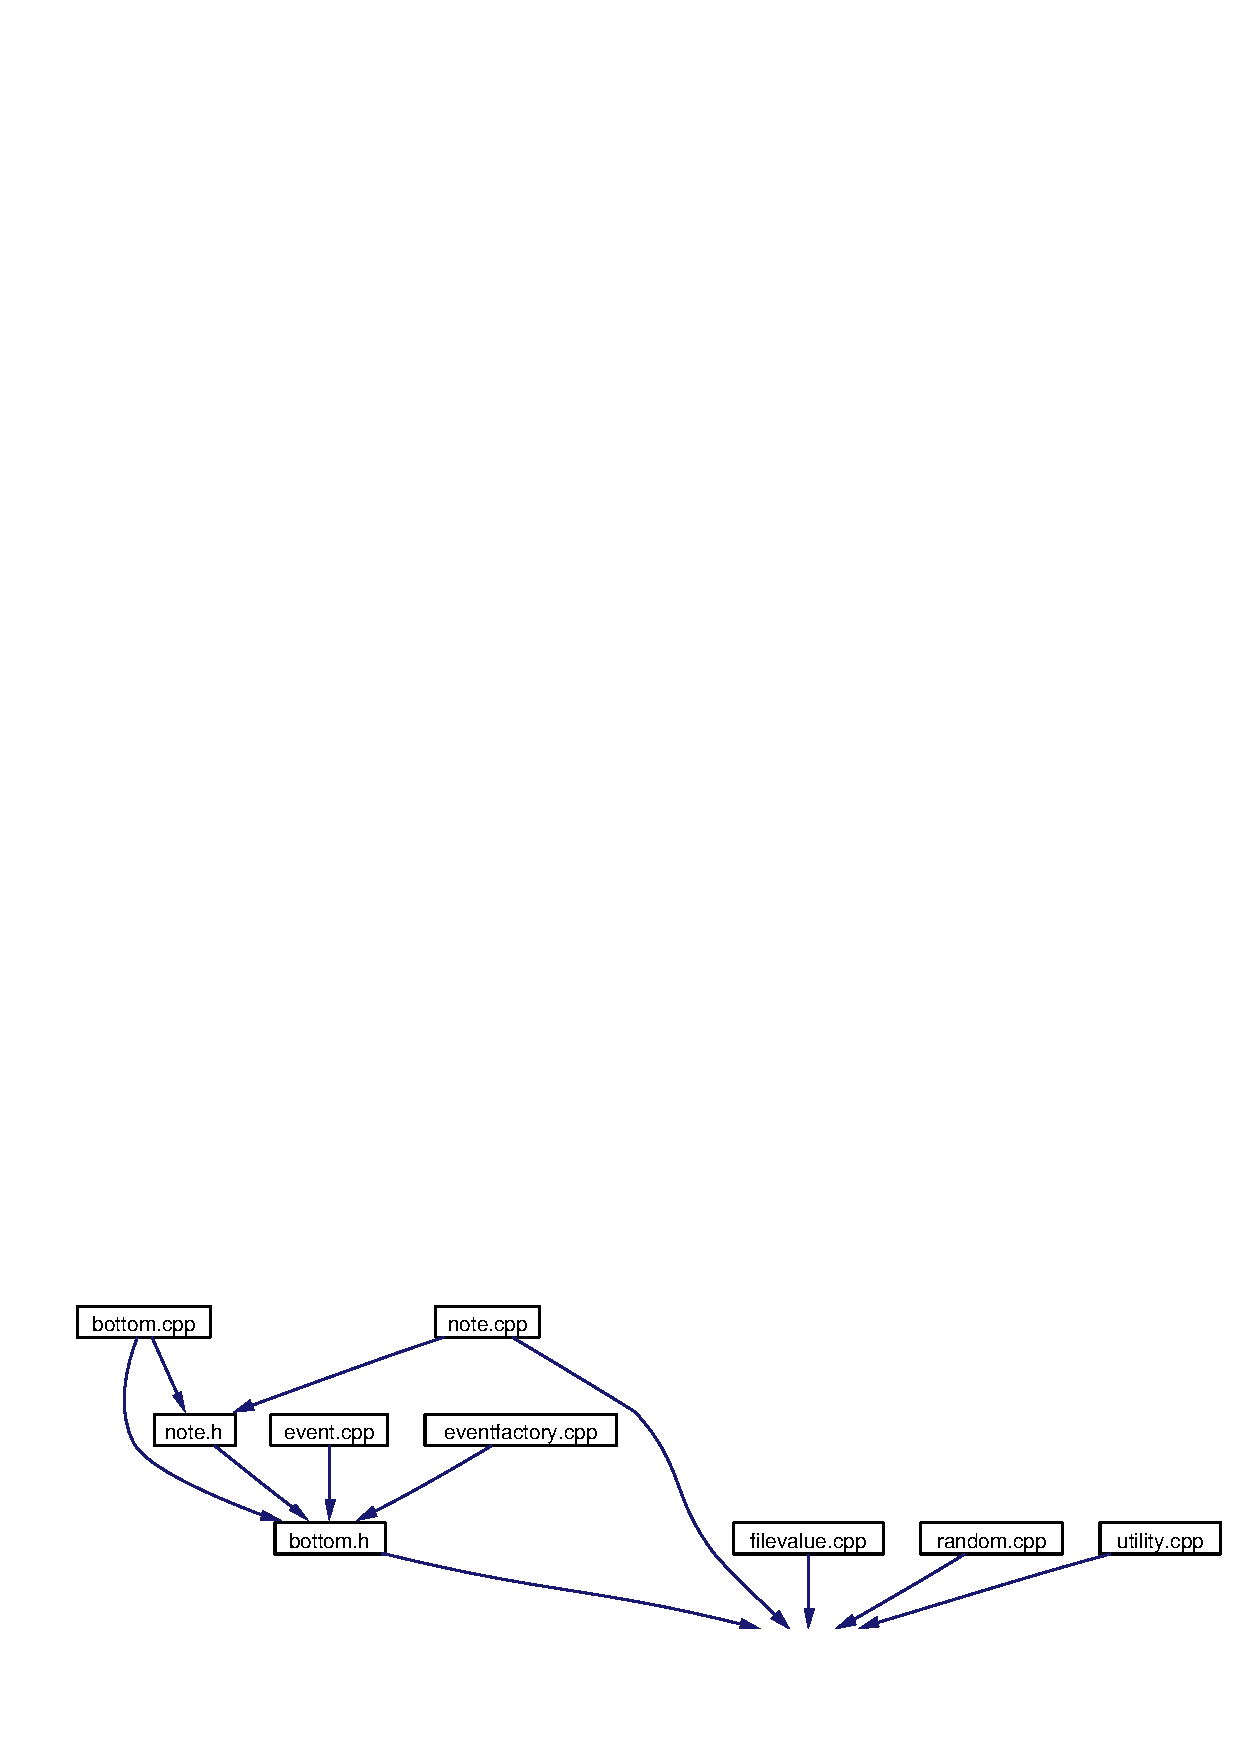
\includegraphics[width=293pt]{define_8h__dep__incl}
\end{center}
\end{figure}
\subsection*{Defines}
\begin{CompactItemize}
\item 
\#define {\bf DEBUG}\ cout
\item 
\#define {\bf NYQUIST}\ 22050.0L
\item 
\#define {\bf CEILING}\ 15000.0L
\item 
\#define {\bf MINFREQ}\ 20.0L
\item 
\#define {\bf TRUE}\ 1
\item 
\#define {\bf FALSE}\ 0
\item 
\#define {\bf PI}\ 4.0$\ast$atan(1.0)
\end{CompactItemize}
\subsection*{Typedefs}
\begin{CompactItemize}
\item 
typedef int {\bf BOOL}
\end{CompactItemize}
\subsection*{Variables}
\begin{CompactItemize}
\item 
const  double {\bf GOLDENMEAN} = 0.618
\item 
const  float {\bf MIN\_\-AUD\_\-FREQ} = 20.
\item 
const  float {\bf MAX\_\-AUD\_\-FREQ} = 20000.
\item 
const  float {\bf FUNDAMENTAL} = 13.75
\item 
const  double {\bf C0} = 16.351597
\item 
const  double {\bf WELL\_\-TEMP\_\-INCR} = pow(2, 1./12.)
\item 
const  float {\bf MAX\_\-SONES} = 256.
\item 
const  float {\bf FIRST\_\-CONST} = -5.54
\item 
const  float {\bf SECOND\_\-CONST} = -1.84
\item 
const  int {\bf SAMPLING\_\-RATE} = 44100
\item 
const  int {\bf DEFAULT\_\-START\_\-TIME} = 0
\item 
const  int {\bf DEFAULT\_\-DURATION} = 1
\end{CompactItemize}


\subsection{Define Documentation}
\index{define.h@{define.h}!CEILING@{CEILING}}
\index{CEILING@{CEILING}!define.h@{define.h}}
\subsubsection{\setlength{\rightskip}{0pt plus 5cm}\#define CEILING\ 15000.0L}\label{define_8h_a2}




Definition at line 46 of file define.h.

Referenced by Bottom::build\-Sound(), File\-Value::Evaluate(), Bottom::Num\-Part(), and Bottom::Set\-Frequency().\index{define.h@{define.h}!DEBUG@{DEBUG}}
\index{DEBUG@{DEBUG}!define.h@{define.h}}
\subsubsection{\setlength{\rightskip}{0pt plus 5cm}\#define DEBUG\ cout}\label{define_8h_a0}




Definition at line 40 of file define.h.\index{define.h@{define.h}!FALSE@{FALSE}}
\index{FALSE@{FALSE}!define.h@{define.h}}
\subsubsection{\setlength{\rightskip}{0pt plus 5cm}\#define FALSE\ 0}\label{define_8h_a5}




Definition at line 49 of file define.h.\index{define.h@{define.h}!MINFREQ@{MINFREQ}}
\index{MINFREQ@{MINFREQ}!define.h@{define.h}}
\subsubsection{\setlength{\rightskip}{0pt plus 5cm}\#define MINFREQ\ 20.0L}\label{define_8h_a3}




Definition at line 47 of file define.h.

Referenced by Bottom::build\-Sound(), File\-Value::Evaluate(), and Bottom::Set\-Frequency().\index{define.h@{define.h}!NYQUIST@{NYQUIST}}
\index{NYQUIST@{NYQUIST}!define.h@{define.h}}
\subsubsection{\setlength{\rightskip}{0pt plus 5cm}\#define NYQUIST\ 22050.0L}\label{define_8h_a1}




Definition at line 45 of file define.h.\index{define.h@{define.h}!PI@{PI}}
\index{PI@{PI}!define.h@{define.h}}
\subsubsection{\setlength{\rightskip}{0pt plus 5cm}\#define PI\ 4.0$\ast$atan(1.0)}\label{define_8h_a6}




Definition at line 50 of file define.h.\index{define.h@{define.h}!TRUE@{TRUE}}
\index{TRUE@{TRUE}!define.h@{define.h}}
\subsubsection{\setlength{\rightskip}{0pt plus 5cm}\#define TRUE\ 1}\label{define_8h_a4}




Definition at line 48 of file define.h.

\subsection{Typedef Documentation}
\index{define.h@{define.h}!BOOL@{BOOL}}
\index{BOOL@{BOOL}!define.h@{define.h}}
\subsubsection{\setlength{\rightskip}{0pt plus 5cm}typedef int {\bf BOOL}}\label{define_8h_a7}




Definition at line 36 of file define.h.

\subsection{Variable Documentation}
\index{define.h@{define.h}!C0@{C0}}
\index{C0@{C0}!define.h@{define.h}}
\subsubsection{\setlength{\rightskip}{0pt plus 5cm}const double {\bf C0} = 16.351597\hspace{0.3cm}{\tt  [static]}}\label{define_8h_a12}




Definition at line 65 of file define.h.\index{define.h@{define.h}!DEFAULT_DURATION@{DEFAULT\_\-DURATION}}
\index{DEFAULT_DURATION@{DEFAULT\_\-DURATION}!define.h@{define.h}}
\subsubsection{\setlength{\rightskip}{0pt plus 5cm}const int {\bf DEFAULT\_\-DURATION} = 1\hspace{0.3cm}{\tt  [static]}}\label{define_8h_a19}




Definition at line 75 of file define.h.\index{define.h@{define.h}!DEFAULT_START_TIME@{DEFAULT\_\-START\_\-TIME}}
\index{DEFAULT_START_TIME@{DEFAULT\_\-START\_\-TIME}!define.h@{define.h}}
\subsubsection{\setlength{\rightskip}{0pt plus 5cm}const int {\bf DEFAULT\_\-START\_\-TIME} = 0\hspace{0.3cm}{\tt  [static]}}\label{define_8h_a18}




Definition at line 74 of file define.h.\index{define.h@{define.h}!FIRST_CONST@{FIRST\_\-CONST}}
\index{FIRST_CONST@{FIRST\_\-CONST}!define.h@{define.h}}
\subsubsection{\setlength{\rightskip}{0pt plus 5cm}const float {\bf FIRST\_\-CONST} = -5.54\hspace{0.3cm}{\tt  [static]}}\label{define_8h_a15}




Definition at line 69 of file define.h.\index{define.h@{define.h}!FUNDAMENTAL@{FUNDAMENTAL}}
\index{FUNDAMENTAL@{FUNDAMENTAL}!define.h@{define.h}}
\subsubsection{\setlength{\rightskip}{0pt plus 5cm}const float {\bf FUNDAMENTAL} = 13.75\hspace{0.3cm}{\tt  [static]}}\label{define_8h_a11}




Definition at line 64 of file define.h.\index{define.h@{define.h}!GOLDENMEAN@{GOLDENMEAN}}
\index{GOLDENMEAN@{GOLDENMEAN}!define.h@{define.h}}
\subsubsection{\setlength{\rightskip}{0pt plus 5cm}const double {\bf GOLDENMEAN} = 0.618\hspace{0.3cm}{\tt  [static]}}\label{define_8h_a8}




Definition at line 61 of file define.h.\index{define.h@{define.h}!MAX_AUD_FREQ@{MAX\_\-AUD\_\-FREQ}}
\index{MAX_AUD_FREQ@{MAX\_\-AUD\_\-FREQ}!define.h@{define.h}}
\subsubsection{\setlength{\rightskip}{0pt plus 5cm}const float {\bf MAX\_\-AUD\_\-FREQ} = 20000.\hspace{0.3cm}{\tt  [static]}}\label{define_8h_a10}




Definition at line 63 of file define.h.\index{define.h@{define.h}!MAX_SONES@{MAX\_\-SONES}}
\index{MAX_SONES@{MAX\_\-SONES}!define.h@{define.h}}
\subsubsection{\setlength{\rightskip}{0pt plus 5cm}const float {\bf MAX\_\-SONES} = 256.\hspace{0.3cm}{\tt  [static]}}\label{define_8h_a14}




Definition at line 68 of file define.h.\index{define.h@{define.h}!MIN_AUD_FREQ@{MIN\_\-AUD\_\-FREQ}}
\index{MIN_AUD_FREQ@{MIN\_\-AUD\_\-FREQ}!define.h@{define.h}}
\subsubsection{\setlength{\rightskip}{0pt plus 5cm}const float {\bf MIN\_\-AUD\_\-FREQ} = 20.\hspace{0.3cm}{\tt  [static]}}\label{define_8h_a9}




Definition at line 62 of file define.h.\index{define.h@{define.h}!SAMPLING_RATE@{SAMPLING\_\-RATE}}
\index{SAMPLING_RATE@{SAMPLING\_\-RATE}!define.h@{define.h}}
\subsubsection{\setlength{\rightskip}{0pt plus 5cm}const int {\bf SAMPLING\_\-RATE} = 44100\hspace{0.3cm}{\tt  [static]}}\label{define_8h_a17}




Definition at line 71 of file define.h.\index{define.h@{define.h}!SECOND_CONST@{SECOND\_\-CONST}}
\index{SECOND_CONST@{SECOND\_\-CONST}!define.h@{define.h}}
\subsubsection{\setlength{\rightskip}{0pt plus 5cm}const float {\bf SECOND\_\-CONST} = -1.84\hspace{0.3cm}{\tt  [static]}}\label{define_8h_a16}




Definition at line 70 of file define.h.\index{define.h@{define.h}!WELL_TEMP_INCR@{WELL\_\-TEMP\_\-INCR}}
\index{WELL_TEMP_INCR@{WELL\_\-TEMP\_\-INCR}!define.h@{define.h}}
\subsubsection{\setlength{\rightskip}{0pt plus 5cm}const double {\bf WELL\_\-TEMP\_\-INCR} = pow(2, 1./12.)\hspace{0.3cm}{\tt  [static]}}\label{define_8h_a13}




Definition at line 66 of file define.h.